% APRESENTACAO DO SERGIO ALONSO - Workshop FISIOCOMP 12-05-2017

\documentclass[unknownkeysallowed]{beamer}
\usepackage[utf8]{inputenc}
\usepackage[brazil]{babel}
\usepackage{beamerthemeCambridgeUS}
\usepackage{graphicx}
\usepackage{multirow}
\usepackage{hyperref}


\title{Study of Bifurcations on Purkinje Fibers}
\author{Lucas Berg}
\date{\today}

\begin{document}
    \maketitle
    
    \begin{frame}
	  \frametitle{Summary}
	  \tableofcontents[section,subsection]
	  \section{Purkinje Fibers}
	  \section{Source-Sink Problem}
	  \section{Under Development}
    \end{frame}
    
    \begin{frame}{Purkinje Fibers}
	      \begin{figure}
		      % During the contraction of heart a specialized set of fibers, known as Purkinje Fibers, conduct the stimulus from the SA
		      % node to the ventricles. This conduction must be always synchronized, so any problems happen in these structures could lead to a desynchronized cardiac rhythim and worst, to a sudden death. 
		      %  
		      \centering
		      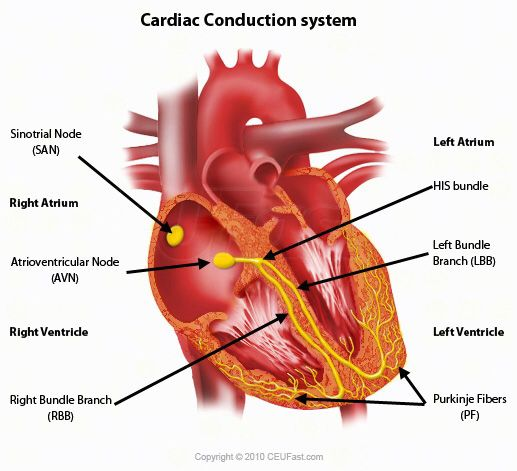
\includegraphics[scale=0.5]{img/cardiac-conduction-system.jpg}
	      \end{figure}
    \end{frame}
    
    \begin{frame}{Source-Sink Problem}
      \begin{itemize}
	      % Retirado de: Remodeling of cardiac passive electrical properties and susceptibility to Ventricular and Atrial Arrhythmias
	      \item When an action potential (AP) propagates in cardiac tissue, the wavefront acts as a source of depolarizing current for the adjacent repolarized tissue (the sink). \newline
	      
	      \item The source current density must be sufficient to bring the sink to its activation threshold, and propagation will fail if the source-sink mismatch is too large. This topic has been extensively studied in both normal and diseased heart for propagating wavefronts  \newline
	      
	      \item In order to elicit an action potential in a cell, it must receive a depolarizing current from an adjacent, activated cell. The activated cell acts as current source, while the non-activated cell us a current sink with the voltage difference being the driving force for this current. The current transfer is mainly realized via gap junction channels and, to some extent, via the extracellular space. 
      \end{itemize}
    \end{frame}
    
    \begin{frame}{Source-Sink Problem}
	    \begin{itemize}
	    \item Whether enough current can be tranferred to activate a cell is a complex and geometric problem: if a small source (e.g., a tiny strand of activated cardiomyocytes) meets a large sink (e.g., a large area of non-activated site to many non-activated cardiomyocites) the current will flow radially from the activated site to many non-activated sites. \newline
	    
	    \item Hence, the source current is distributed to many neighboring cells and in each of these the accumulated charge may be too low to trigger an action potential. This will cause conduction failure.
	    \end{itemize}
    \end{frame}
    
    \begin{frame}{Source-Sink Problem}
	   \begin{itemize}
	    \item Situations with source-sink problems generally occur when the curvature of the propating wave front is high. Accordingly, they may be found at the end of Pukinje Fibers, during propagation through small isthmuses, around obstacles, and during spiral wave re-entry. \newline
	    	    
 	    \item Furthermore, source-sink mismatch may occur at the border between normal cardiac tissue and an ischemic zone, when depolarizing current flows into the ischemic region. Since this region is usually non-excitable, it will act as a current sink, consenquently, reduce conduction velocity.
 	   \end{itemize}
    \end{frame}
    
    \begin{frame}{Source-Sink Problem}
	    COLOCAR UMA FIGURA
    \end{frame}
    
    \begin{frame}{Under Development}
	    \begin{itemize}
		    \item \textbf{Objective:} study how bifurcations on Purkinje Fibers affect the source-sink mismatch. \newline
		    \item \textbf{Equation:} Monodomain \newline
		    \item \textbf{Models:} Noble (1962) and Li \& Rudy (2011) \newline
		    \item \textbf{Methods to use:} Finite Volumes and Finite Elements \newline
		    \item \textbf{Parameters to analyze:}
		    \begin{itemize}
			    \item Number of bifurcations. 
			    \item Propagation velocity. 
			    \item Size of the fibers. 
			    \item Size of the discretization in space.
			\end{itemize}
	    \end{itemize}
    \end{frame}
    
    \begin{frame}{Under Development}
	    COLOCAR UMA FIGURA (Bif 4 e Bif 40)
    \end{frame}
\end{document} 


